\documentclass[czech]{ExcelAtFIT}
%\documentclass[czech]{ExcelAtFIT} % when writing in CZECH
%\documentclass[slovak]{ExcelAtFIT} % when writing in SLOVAK
\usepackage{listings}
\definecolor{lightgray}{rgb}{.9,.9,.9}
\definecolor{darkgray}{rgb}{.4,.4,.4}
\definecolor{purple}{rgb}{0.65, 0.12, 0.82}
\lstdefinelanguage{PHP}{
  keywords={instanceof, void, new, true, false, catch, function, return, null, switch, AND, var, if, while, do, for, else, as, elseif, case, break, include, require, foreach, echo},
  keywordstyle=\color{blue}\bfseries,
  ndkeywords={class, extend, implements, array, bool, int, string, float, throw, this},
  ndkeywordstyle=\color{darkgray}\bfseries,
  identifierstyle=\color{black},
  sensitive=false,
  comment=[l]{//},
  morecomment=[s]{/*}{*/},
  commentstyle=\color{purple}\ttfamily,
  stringstyle=\color{red}\ttfamily,
  morestring=[b]',
  morestring=[b]"
}

\lstset{
   language=PHP,
   backgroundcolor=\color{lightgray},
   extendedchars=true,
   basicstyle=\footnotesize\ttfamily,
   showstringspaces=false,
   showspaces=false,
   numbers=left,
   numberstyle=\footnotesize,
   numbersep=9pt,
   tabsize=2,
   breaklines=true,
   showtabs=false,
   captionpos=b
}

\renewcommand{\lstlistingname}{Kód}
\newcommand{\function}[1]{\texttt{#1}}

\def\UrlBreaks{\do\/\do-}

%--------------------------------------------------------
%--------------------------------------------------------
%	REVIEW vs. FINAL VERSION
%--------------------------------------------------------

%   LEAVE this line commented out for the REVIEW VERSIONS
%   UNCOMMENT this line to get the FINAL VERSION
%\ExcelFinalCopy


%--------------------------------------------------------
%--------------------------------------------------------
%	PDF CUSTOMIZATION
%--------------------------------------------------------

\hypersetup{
	pdftitle={Překlad podmnožiny jazyka PHP do C++},
	pdfauthor={Stanislav Nechutný},
	pdfkeywords={PHP, C++, Translation, Module}
}


%--------------------------------------------------------
%--------------------------------------------------------
%	ARTICLE INFORMATION
%--------------------------------------------------------

\ExcelYear{2016}

\PaperTitle{Překlad podmnožiny jazyka PHP do C++}

\Authors{Stanislav Nechutný*}
\affiliation{*
  \href{mailto:xnechu01@stud.fit.vutbr.cz}{xnechu01@stud.fit.vutbr.cz},
  \textit{Faculty of Information Technology, Brno University of Technology}}

\Keywords{PHP --- C++ --- Překlad --- Rozšíření}

\Supplementary{\href{https://www.github.com/nechutny/BP}{Zdrojový kód}}


%--------------------------------------------------------
%--------------------------------------------------------
%	ABSTRACT and TEASER
%--------------------------------------------------------

\Abstract{

Tato práce se zaměřuje na návrh a tvorbu nástroje pro automatizovaný překlad funkcí napsaných v~podmnožině jazyka PHP do C++. Vygenerovaný zdrojový kód je možno zkompilovat jako rozšíření PHP a zavést stejným způsobem, jako například MySQL, PDO, GD apod. Ve výsledku je tedy možno zavolat tyto funkce z~PHP, jako by se jednalo o~původní interpretovanou funkci. Předpokladem je však rozdíl v~rychlosti vykonávání, protože odpadá analýza zdrojových kódů, jejich interpretace, či režie způsobená správou paměti. Vytvořený nástroj provádí převod zdrojového kódu do abstraktního syntaktického stromu, staticky jej analyzuje pro určení datových typů proměnných a následně provádí generování C++ kódu.

%This papper focus on development of tool for automated translation functions written in PHP 5.6 language into C++ source. Targeted output source code should be compiled as PHP extension module and loaded in the same way as MySQL PDO, GD etc. So in result we can call these functions from PHP as originals, but is expected faster execution, because we don't need more to parse and interpret source plus garbage collector is no more needed. Developed tool parse input source into abstract syntactic tree and analyze them for determining variable types and generate output code.

%\todo{What is the problem? What is the topic?, the aim of this paper?}

%\todo{How is the problem solved, the aim achieved (methodology)?}

\todo{What are the specific results? How well is the problem solved?}

\todo{So what? How useful is this to Science and to the reader?}
}

%\Teaser{
%	\TeaserImage{placeholder.pdf}
%	\TeaserImage{placeholder.pdf}
%	\TeaserImage{placeholder.pdf}
%}



%--------------------------------------------------------
%--------------------------------------------------------
%--------------------------------------------------------
%--------------------------------------------------------
\begin{document}

\startdocument


%--------------------------------------------------------
%--------------------------------------------------------
%	ARTICLE CONTENTS
%--------------------------------------------------------

%--------------------------------------------------------
%--------------------------------------------------------
%--------------------------------------------------------
%--------------------------------------------------------
\section{Úvod}

	%\textbf{[Motivation (9 lines)]}
		%\phony{What is the raison d'\^{e}tre of your project? Why should anyone care? No general meaningless claims. Make bulletproof arguments for the importance of your work.}

		Současné webové aplikace napsané v~PHP obsahují desítky knihoven, které programátoři nepotřebují upravovat a chtějí je jen použít. Tyto knihovny někdy provádějí výpočetně náročné operace. Jelikož jsou interpretovány, tak dochází k~zpomalení v~důsledku použitých mechanismů. Příkladem je správa paměti, která může způsobovat výrazné zpomalení. Na tuto skutečnost poukázala optimalizace nástroje Composer, které bylo dosaženo vypnutím automatického u\-vol\-ňo\-vá\-ní nepoužívané paměti a dosáhla 30\% - 90\% zrych\-lení (v~závislosti na množství prováděných operací)\cite{gcOptimize}. Dlouhá doba načítání webové stránky je jedním z~hlav\-ních důvodů pro opuštění návštěvníkem. Škálování takových náročných systémů pak nemusí být e\-ko\-no\-mic\-ké řešení. Tento nástroj však umožňuje snížit vytížení serverů s~nutností minimální úpravy aplikace.

		%Current web applications written in PHP contains tens of libraries, which programmer doesn't need to modify and just use them. These libraries sometime consume a lot of processor time, because are interpreted and are used other mechanisms from scripting language eg. garbage collector\cite{gcOptimize}. Web application response time is for costumer one of main reason to leave it, and scaling such systems is not economic solution. This solution allow to decrease servers load with minimal need of application modification.

	%\textbf{[Problem definition (17 lines)]}
		 %\phony{What exactly are you solving? What is the core and what is a bonus? What parameters should a proper solution of the problem have? Define the problem precisely and state how its solution should be evaluated.}

		Překlad zdrojového kódu z~dynamicky typovaného jazyka do silně typovaného je problematický hned z~několika důvodů. Prvním je detekce datových typů ze zdrojového kódu. Dále tu máme různé obtížně přeložitelné konstrukce, jako například potlačení chybového výpisu, či operátor porovnání.

		%Translating source code from dynamicly typed scripting language to strongly typed compiled code is problematic in a lof of ways. One of the main problems is detecting variable types from source code. Next we have a lot of not so easily translatable constructions such as warning supression, space ship operator etc.

		Prvně je třeba provést syntaktickou analázu zdrojových kódů a převést je do abstraktního syntaktického stromu pro následnou analýzu. Na základě této struktury můžeme provést analýzu možných hodnot, graf volání apod. pro detekci datových typů. Toto řešení však nepokrývá veškeré možnosti, takže v~projektu jsem také experimentoval s~generováním kódu pro více variant a následnou volbou vykonaného kódu za běhu na základě obdržených hodnot.

		%Firstly we need to parse existing source and tranform it into abstract syntactic tree for futher analysation. Based on this structure we can analyse varible possible values, call graphs etc. to determine data types. This solution doesn't cover all possibilities, so in this project we are also experimenting with generating code for more types and choosing execution tree at run-time.

		%Poslední část tohoto článku se zabývá porovnáním výkonu přeloženého kódu s~originálním kódem v~PHP \todo{Stihnu?} a problémy s~některými konstrukcemi.

		%Last part of this article focus on benchmark tests of translated code and problems with some constructions.



	%\textbf{[Existing solutions (23 lines)]}
		%\phony{Discuss existing solutions, be fair in identifying their strengths and weaknesses. Cite important works from the field of your topic. Try to define well what is the \textit{state of the art}. You can include a Section 2 titled ``Background'' or ``Previous Works'' and have the details there and make this paragraph short. Or, you can enlarge this paragraph to a whole page. In many scientific papers, \emph{this} is the most valuable part if it is written properly.}

		V~současné době zde není přímo konkurenční řešení. Můžeme porovnat tento projekt s~HPHPc od společnosti Facebook, které však bylo zamýšleno pro kompilaci celé PHP aplikace do jednoho velkého binárního sou\-bo\-ru. Toto je rozdílný koncept, jelikož HPHPc vy\-ža\-do\-va\-lo překompilování celé aplikace i v~případě drobné změny a následnou distribuci až několik GB velkého souboru na servery. Představené řešení je však zaměřeno pouze na kompilaci knihoven, které nejsou měněny často a hlavní aplikace je stále interpretována. Projekt HPHPc byl nahrazen projektem HHVM\footnote{\url{http://hhvm.com/}}, který je JIT kompilátor spouštějící bytecode ve virtálním stroji, čímž řeší zmíněné nedostatky HPHPc\cite{hphpcHipHop}.


		%In current time there isn't direct competitive solution. We can compare this project with Facebook's project HPHPc which intended to compile whole PHP application into one binary executable. This is different concept, because HPHPc's implementation require recompiling application even when was changed only few lines of file and then redistribute eventualy a few gigabites large binary files. This solution is intended to compile just libraries, when they are not changed so often and main application using these libraries is still interpreted. HPHPc project was replaced with HHVM that is Just In Time compiler runing in Virtual Machine which solve problems with recompiling.

		Dále existuje projekt PHC\footnote{\url{http://www.phpcompiler.org/}}, který také kompiluje PHP aplikaci do spustitelného binárního souboru a má experimentální podporu pro generování rozšíření PHP. Bohužel se mi nepodařilo tuto funkcionalitu otestovat, protože kód již není delší dobu udržován a nepodařilo se mi jej zkompilovat na Debian stable s~PHP 5.3 i přes různé úpravy kódu.

		%There is also project PHC that compile too php application into executable binary, but have experimental support for creating php extensions from php code. This feauture can't be tested, because code is no more maintained and I was unable to compile it even not on debian stable with PHP 5.3 and some code changes.

		Většina zbylých řešení ve výsledku pouze zabalí PHP skript do datové části spustitelného souboru a přibalí PHP interpret. Nejedná se tedy de facto o~pře\-kla\-dač, ale o~pouhé zabalení skriptu k~interpretru.

		%Most of other solutions in fact just pack php script into data part of executable containing PHP and interpret it when executed.

	%\textbf{[Our solution (13 lines)]}
		%\phony{Make a quick outline of your approach -- pitch your solution.  The solution will be described in detail later, but give the reader a very quick overview now.}

		Zde zmiňované řešení používá funkce z~PHP pro převod zdrojového kódu na tokeny a přidává další vrstvu abstrakce pro přesnější rozlišení tokenů. Pro parsování zdrojových kódů je použit vlastní parser s~rekurzivním sestupem a zásobníková precedenční analýza. Vlastní řešení bylo zvoleno pro snadnost úpravy, získání veškerých potřebných údajů v~po\-ža\-do\-va\-ném formátu a vyzkoušení si teorie v~praxi.

		%This solution use PHP's functions for tokenizing source code and have added abstract layer for more precise token detection, own recursive parser, stack precedence analysator. Own solution was chosen because of optimizating gather informations.

		Abstraktní syntaktický strom z~precedenční analýzy je použit pro zjištění použitých proměnných a operací s~nimi prováděných. Dvěma průchody stromu jsou na základě prováděných operací a volaných funkcí přiřazeny proměnným datové typy. Současně s~par\-so\-vá\-ním a precedenční analýzou probíhá také předávání informací generátorům, které mají na starosti výsledný C++ kód.

		Po úspěšném rozparsování a zanalyzování zdrojového kódu je provedeno generování kódu na základě zjištěných informací,


	%\textbf{[Contributions (7 lines)]}
		%\phony{Sell your solution. Pinpoint your achievements. Be fair and objective.}
		Nástroj, jehož návrh a implemetace je v~tomto článku popisována, je možnost, jak dosahnout snadno rychlejší odezvy PHP aplikací. V~současné době je praktické použití komplikované implementací pouhé podmnožiny jazyka PHP a zejména absence objektové části je pro překlad moderních knihoven problematická. To však vzhledem k~pokračujícímu vývoji nemusí být překážkou nastálo.





%--------------------------------------------------------
%--------------------------------------------------------
%--------------------------------------------------------
%--------------------------------------------------------

\section{Teorie}

	Některé knihovny jsou náročné na výpočet a i přesto implementovány v~PHP pro jeho jednoduchost na psaní a velký rozsah funkcí, kdy se není třeba zaměřovat na správu paměti, čtení ze souboru apod. Cílem je ponechat tuto jednoduchost a přinést zrychlení. Pří\-kla\-dem může být rozpoznání obličeje\footnote{\url{https://github.com/mauricesvay/php-facedetection}}, nebo generování PDF z~HTML - mPdf.

	Optimalizace přepisováním částí systému do C/C++ není zcela běžná, ale používá se u~velkých projektů - třeba Yahoo provádí přepisování náročných částí aplikace do C++\cite{yahooCpp}. Z~open source knihoven pak může být příkladem framework Phalcon\footnote{\url{https://phalconphp.com/en/}}, či Ice, které jsou kompletně napsané v~jazyce C. Zpřístupňují MVC model s~databázovou vrstvou, šablonami a dalšími funkcemi, jako klasické frameworky implementované v~PHP. Dle testů\cite{phalconBenchmark} webová aplikace využívající výhod této optimalizace je schopna odbavit násobky pří\-cho\-zích požadavků oproti implementacím v~PHP. Je tedy zřejmé, že tato optimalizace má smysl a právě cílem této práce je zjednodušit tvorbu C++ knihoven pro PHP.


	Životní cyklus PHP rozšíření sestává z~několika stavů.\cite{phpExtensionLife} Při startu PHP jsou načteny sdílené knihovny definované v~konfiguračním souboru direktivou \function{ex\-ten\-sion=}, a zavolána funkce vracející informace o~rozšíření. Tyto informace obsahují verzi PHP API, callbacky a funkce, třídy, rozhraní a konstanty, které rozšíření poskytuje.\cite{phpExtensionStructure}

	Po inicializaci PHP jsou zavolány inicializační funkce rozšířeních, které umožňují provést alokaci paměti, otevření deskriptorů k~souborům apod. V~tomto kroku je například vhodné, aby rozšíření pro logování otevřelo soubor, do kterého bude zapisovat, jelikož bude pro všechny požadavky stejný a je zbytečné jej otevírat a zavírat při každém požadavku.

	PHP proces čeká na pří\-cho\-zí požadavek k~odbavení. Při jeho přijetí nastaví potřebné proměnné a spustí interpretaci skriptu. Spolu s~nastavením proměnných je zavolán další callback z~rozšíření, který může připravit k~načtení již konkrétní hodnoty pro daný požadavek - může tím být například vlastní implementace session.

	\begin{figure}[t]
		\centering
		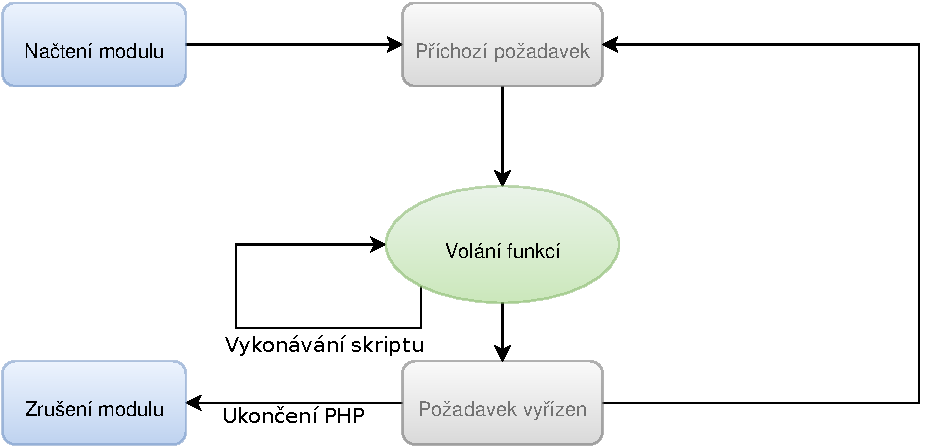
\includegraphics[width=1.0\linewidth]{PhpExtensionLifeCycleDiagram.pdf}
		\caption{Životní cyklus PHP rozšíření.}
		\label{fig:phpExtensionLifeCycle}
	\end{figure}


	Následně dochází k~případným voláním funkcí při vykonávání skriptu obsluhujícího požadavek. Po dokončení požadavku je zavolán další callback, který umožňuje provést uvolnění paměti a další operace pro funkcionalitu rozšíření. Z~důvodu optimalizace nedochází po obsloužení požadavku k~ukončení procesu PHP, ale proces čeká na další příchozí požadavek. Pokud dojde k~vypnutí webového serveru, tak je zavolán další callback, který by měl provést úklid zbylých zdrojů - protiklad k~prvně volanému callbacku. Celý tento proces znázorňuje diagram na obrázku č. \ref{fig:phpExtensionLifeCycle}.


	Z~PHP rozšíření není možné ovlivňovat seznam vložených souborů pro funkce \function{include\_once} a \function{re\-qui\-re\_on\-ce}. Pokud bude přeložen zdrojový kód vkládající část pomocí jedné z~těchto funkcí, tak v~době vykonávání bude možné provést opět jedno vložení souboru, který byl vložen v~přeloženém kódu.

	Velmi problematickým je pak překlad konstrukcí jako \function{\$\$varName}, které v~jazyce PHP zpřístupní pro\-měn\-nou, jejíž název je uložen v~proměnné \function{\$varName}. Vzhledem k~tomu, že hodnota proměnné může být předána jako argument funkce, či načtena ze souboru a nemusí být v~době překladu známa, se jedná o~velmi problematickou konstrukci, která není v~současné implementaci podporována.




\section{Definice}

	Při návrhu nástroje bylo třeba vybrání vhodné pod\-mno\-žin\-y PHP k~implemetaci. Vzhledem k~rozsahu nebylo možné za omezený čas implementovat podporu kompletní gramatiky jazyka. Vybraná podmnožina by měla umožnit tvorbu funkcí, volání funkcí a řízení toku programu. Tedy implementovat konstrukce pro podmínky, cykly a zaměřit se zejména na podporu výrazů, která je klíčová. Při transformaci výrazů mezi těmito jazyky je třeba řešit odlišnosti v~prioritě a chování některých operátorů.

	V~současné době neimplementovanou, ale v~budoucnu plánovanou funkcionalitou je podpora objektového programování - tj. podpora pro třídy, dědičnost, rozhraní, jmenné prostory, mixins apod.

	Nástroj provádí jako jednu ze svých funkcí analýzu výrazů a kódu pro detekci datových typů. Použití C++ třídy s~přetíženými operátory povádějící převod hodnoty do požadovaného typu pro veškeré proměnné by mohlo mít nepříznivý dopad na rychlost, a proto, pokud je to možné, jsou použity primitivní datové typy \function{long}, \function{double}, \function{std::string}, \function{boolean} a \function{std::vector} / \function{std::map}.

\begin{lstlisting}[caption=Podporované výrazy PHP, label=code:phpCodeExample, language=PHP]
function hello($name, array $arg = []) {
	foreach($arg AS $a)
	{
		if(rand() AND 1 ** "15")
		{
			echo "Hello ".$name." -- ".$a;
		}
	}
	return count(str_replace("a","b",$arg));
}
\end{lstlisting}

	Kód \ref{code:phpCodeExample} ukazuje některé podporované konstrukce překladače pro převod z~PHP do jazyka C++ - možnost definovat výchozí hodnotu argumentů, podpora pro mocninu, vyhodnocování výrazů, či volání vestavěných funkcí.

	%- třeba vybrat správnou podmnožinu jazyka, aby z~ní bylo možné sestavit rozumně velké funkce pro testování. Proto se hlavní část zaměřuje na výrazy, kdy je podporována většina operátorů. Zde je třeba řešit spoustu odlišností PHP a C++.

	%- z~důvodu komplexnosti byla vypuštěna objektová část jazyka PHP.

	% - detekce datových typů je podstatná část z~důvodu optimalizace, jelikož režie C++ třídy s~přetíženými operátory provádějící dynamická přetypování je výrazně vyšší, než použtí nativních datových typů jako je double apod.






\section{Experimenty a implementace}

	Před zahájením návrhu a implemetace jsem provedl několik testů pro změření rozdílů doby vykonávání. Na obrázku č. \ref{fig:bubbleSort} můžeme vidět graf ukazující dobu potřebnou pro seřazení stejného pole o~50 000 ná\-hod\-ných číslech algoritmem Bubble sort. Zdrojové kódy obou variant jsou přiloženy u~zdrojového kódu projektu. Výrazný rozdíl časů - 3.42s a 0.24s v~prospěch pro C++ naznačuje, že je možné dosáhnout výrazné optimalizace. V~tomto případě zrychlení 14.24x. Obdobných výsledků hovořících v~prospěch C++ verze zavedené jako rozšíření byly i další experimenty. Uvedu dále například součet všech čísel od 1 do 100 000 000 000, kdy čísla jsou ještě více rozdílná - 73s PHP a 0.35s C++. Tyto testy byly prováděny na počtači s~OS Fedora 21, Intel i7 4702MQ, SSD. Měření bylo provedeno 50x a vypočten matematický průměr. Žádná z~naměřených hodnot nevybočovala výrazněji z~prů\-mě\-ru.

	%- experimentování s~syntetickým kódem (napsaným za účelem testování, není z~reálné aplikace). Přepis do C++ ručně, tedy zřejmě nejoptimálnější verze. Implementace Bubble sortu pro 50 000 stejných náhodných položek PHP: 3.42s, C++: 0.24s tj. 14.25x rychlejší. Součet čísel od 0 do N PHP: 73s, C++: 0.35s \todo{zanést do grafu}.

\begin{figure}[t]
	\centering
	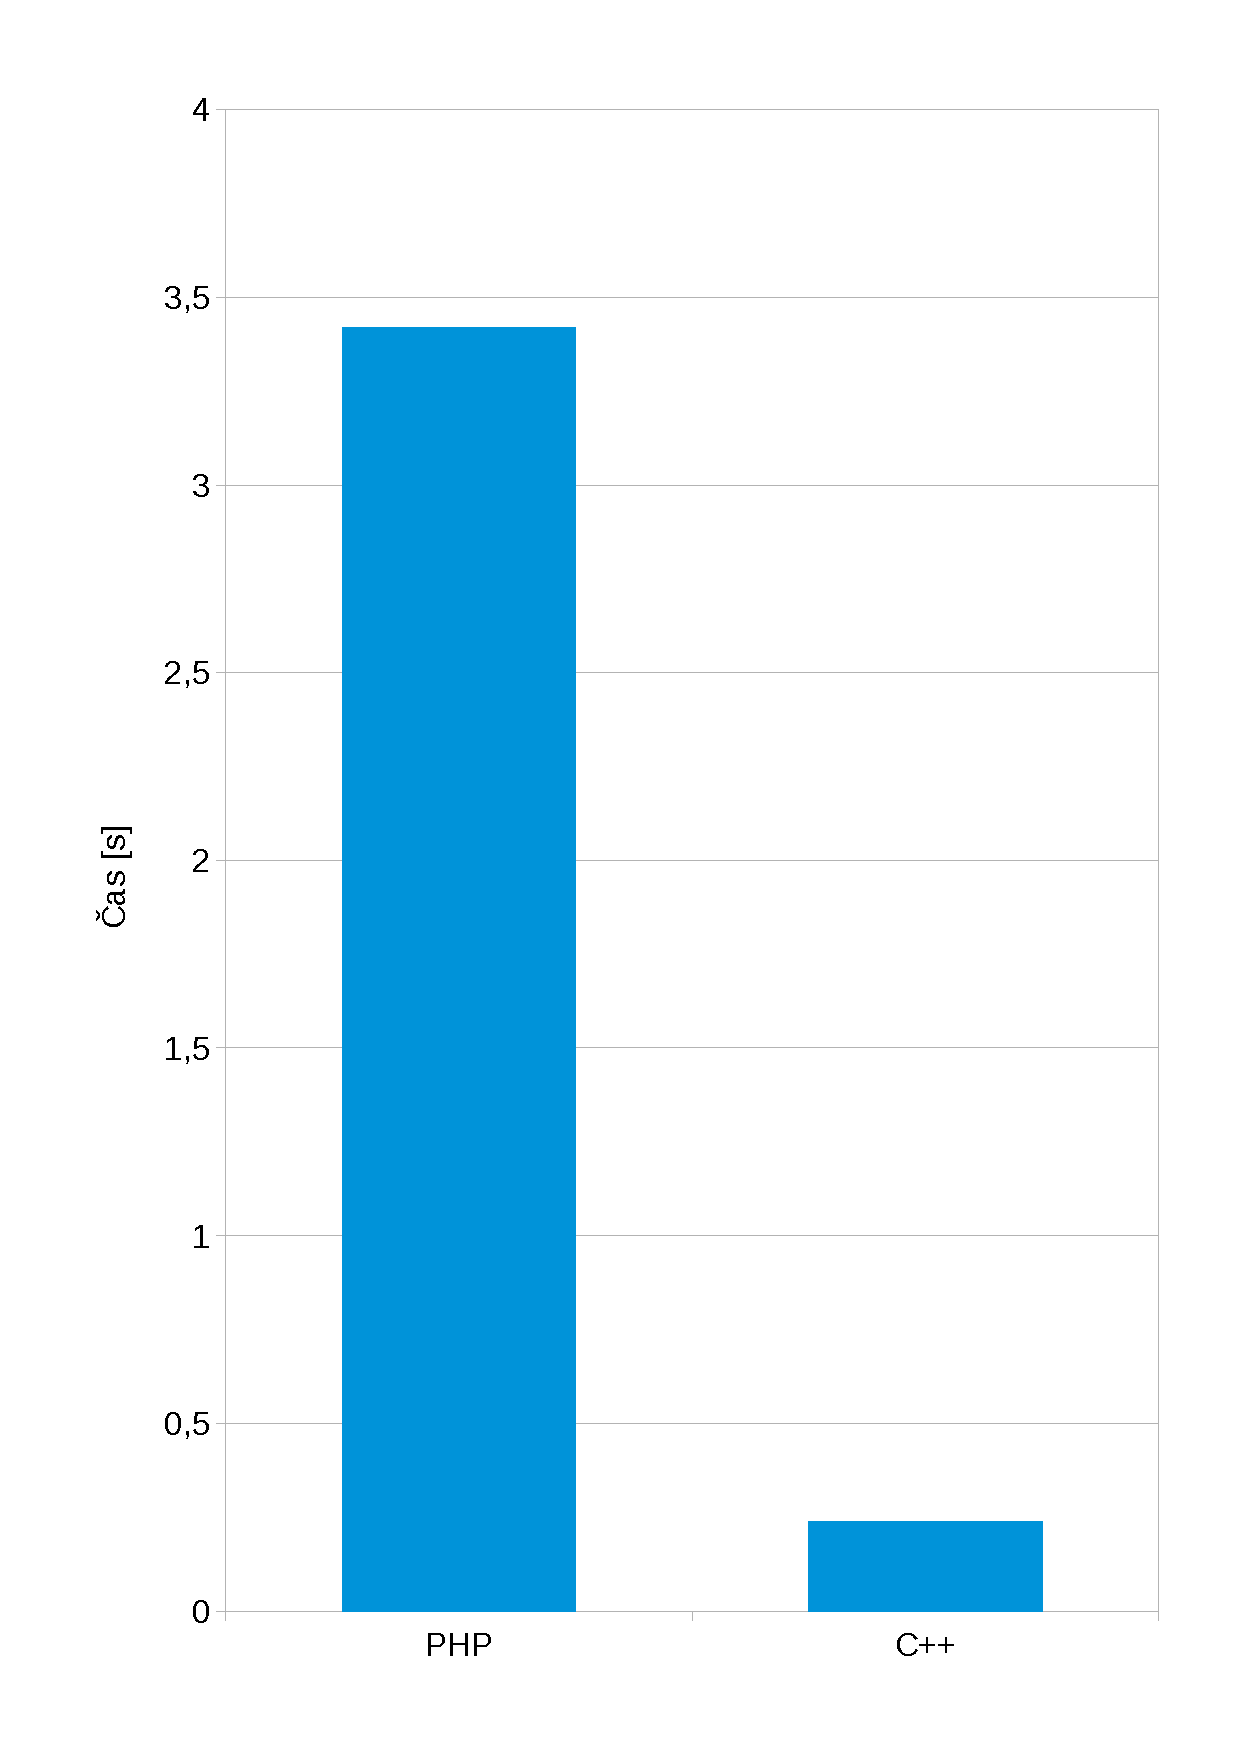
\includegraphics[width=1.0\linewidth]{bubbleSort.pdf}
	\caption{Porovnání rychlosti Bubble sortu.}
	\label{fig:bubbleSort}
\end{figure}

	Zrychlení bude velmi záležet na charakteristice překládaného kódu. V případě, že se bude jednat o pouhá volání vestavěných, či knihovních funkcí, které jsou již zkompilované, tak zrychlení bude maximálně v řádu jednotek procent, či dokonce nulové. Mnohem zajímavějších výsledků je však možno dosahnout v případě funkcí, které provádějí ve větší míře operace s proměnnými, viz výše uvedený Bubble sort.

	Rozšíření je možné implementovat v~C pro\-střed\-nic\-tvím rozhraní definovaného společností Zend, která stojí za referenčním interpretrem PHP. Dokumentace i s~návody je dostupná na jejím webu. Po průzkumu možností jsem zvolil knihovnu PHP-CPP\footnote{\url{http://www.php-cpp.com/}} od spo\-leč\-nos\-ti Copernica, která umožňuje pohodlnější tvorbu PHP rozšíření přidáním abstrakce a zpřístupněním funkcí z~PHP v~prostředí jazyka C++.

	Tato knihovna implementuje třídu \function{Php::Value}, která slouží pro předávání argumentů z~PHP do funkcí implementovaných v jazyce C++ a zpět. Pro samotné použití v~generovaném kódu místo nativních typů není vhodná, jelikož její provázání s~PHP interpretem má vysokou režii.

	Pro tvorbu programu byl zvolen jazyk PHP, který poskytuje prostředky pro rychlý vývoj s~možnostmi provádět rychlé změny v~kódu. Dalším důvodem pro PHP je vestavěný tokenizer pro zdrojový jazyk. Ten bylo třeba rozšířit o~podrobnější kategorizaci tokenů, o~což se stará vlastní lexikální analyzátor.

	Pro tvorbu abstraktního syntaktického stromu z~tokenů je použit vlastní parser s~rekurzivním sestupem. V~průběhu parsování jsou již předávány generátorům kódu informace o~konstrukcích, které mají generovat a prováděna derivace výrazů precedenční analýzou.

	Před samotným generováním C++ kódu dochází k~detekci datových typů. Tato detekce je provedena ve dvou krocích. Při prvním průchodu stromem jsou určeny požadované vstupní typy hodnot do uzlů stromu a výsledná hodnota na základě operátorů. Například při operaci dělení je zřejmé, že výsledkem bude typ float, či u~konkatenace řetězec a jeho operandy budou také řetězec (u~jiných typů se provede přetypování). Obdobně jsou pak určeny typy hodnot - čísla, řetězce, či návratové hodnoty vestavěných funkcí.

	Druhým průchodem tímto stromem s~již částečnými informacemi o~typech jsou doplněny zbylé typy v~zá\-vis\-los\-ti na operacích - pokud je prováděno sčítání dvou hodnot typu int, tak výsledkem bude int. V~případě, že je jedna z~nich typu double, tak již výsledek bude také typu double. V~případě přiřazení do proměnné je tento typ uložen k~proměnné s~adresou značící místo použití typu.

	Pokud se nepodaří detekovat s~jistotou typ pro\-měn\-né, tak je raději zvolen benevoletnější, který umožní uložit všechny možné hodnoty - tedy pro číslo raději double, než int. V~případě úplné neznalosti typu je použita instance třídy \function{Php::Value} z~knihovny PHP-CPP, která má větší režii, ale umožňuje práci s~všemi datovými typy\cite{phpCppPerformance}.

	Při generování C++ kódu jsou řešeny rozdíly mezi C++ a PHP. Průchodem bloků kódu jsou získány všech\-ny použité proměnné a definovány na začátku funkce. Důvodem je rozdílný obor platnosti proměnných. Dále je v~instanci třídy reprezentující proměnnou uloženo od jaké části kódu byla proměnná definována a kde byla zrušena konstrukcí \function{unset}, aby došlo k~nahrazení konstrukce \function{isset} za správnou hodnotu.

	Další generátor je specializovaný pro generování výrazů. Při generování řeší konverzi výsledků pod\-vý\-ra\-zů na datový typ potřebný pro další operace pro\-střed\-nic\-tvím funkcí \function{php2cpp::to\_string} a \function{php2\-cpp\-::to\_\-float} implementovaných v~C++. Dalším ú\-ko\-lem je konverze operátorů chybějících v~C++. Pro operátor mocniny je volána funkce \function{pow} z~matematické knihovny a rozdílné priority operátorů jsou řešeny zá\-vor\-ko\-vá\-ním.

	Volání vestavěných, či uživatelem definovaných funkcí je řešeno pomocí metod z~knihovny PHP-CPP pro provázání s~interpretrem.

	%- Použití knihovny PHP-CPP, popsat jak zjednodušuje vývoj (třída PHP::Value) a naopak zas nevhodnost postavit řešení čistě na ní - pomalost práce s~tímto datovým typem.


	%- implemetace parseru

	%- precedenční analýza

	%- detekce datových typů - operace, hodnoty, přiřazení výsledků, návratové hodnoty vestavěných funkcí, \todo{ typy parametrů vestavěných funkcí? }, dvojí průchod stromem, uložení v~struktuře adresované cestou v~kodu




%--------------------------------------------------------
%--------------------------------------------------------
%--------------------------------------------------------
%--------------------------------------------------------
\section{Závěr}
\label{sec:Conclusions}

	%\textbf{[Paper Summary]} \phony{What was the paper about, then? What the reader needs to remember about it?}

	Konverze PHP knihoven do C++ je možná a použití dává smysl při konverzi knihoven, či jiných neměnných částí. Tento postup je vhodný i při vývoji, kdy testování trvá kratší dobu a je možno měnit kód aplikace.


	%\textbf{[Highlights of Results]} \phony{Exact numbers. Remind the reader that the paper matters.}

	V~případě jednoduššího kódu je výsledný kód vý\-raz\-ně rychlejší, než původní. Pro složitější konstrukce je komplikované určit přesně datové typy a tak nemusí být zrychlení natolik výrazné, aby se vyplatilo s~přihlédnutím k~možnému zavlečení chyby.


	%\textbf{[Paper Contributions]} \phony{What is the original contribution of this work? Two or three thoughts that one should definitely take home.}


	%\textbf{[Future Work]} \phony{ How can other researchers / developers make use of the results of this work?  Do you have further plans with this work? Or anybody else? }

	Jsou dostupné zdrojové kódy pod open source licencí Apache 2.0 umožňující vyzkoušet si překlad a v~případě úspěchu nasadit, či se zapojit do vývoje.

	V~budoucnu je plánována podpora tříd, propracovanější detekce datových typů (nyní je občas použit double i když by stačil long), omezit zbytečná volání \function{to\_string} a \function{to\_float}. Dále je plánováno experimentování s~další detekcí datových typů, kdy slibné výsledky by mohlo poskytnout sledování hodnot pro\-měn\-ných v~interpretované verzi při provozu. Při dos\-ta\-teč\-ně velkém množství vzorků by bylo možné vygenerovat optimalizovanou verzi + obecnou. Při zavolání knihovny by se poté zvolila varianta dle typů argumentů.

%\section*{Acknowledgements}
%I~would like to thank my supervisor X. Y. for his help.

%--------------------------------------------------------
%--------------------------------------------------------
%--------------------------------------------------------
%	REFERENCE LIST
%--------------------------------------------------------
%--------------------------------------------------------
\phantomsection
\bibliographystyle{unsrt}
\bibliography{2016-ExcelFIT-php2cpp-bib}

%--------------------------------------------------------
%--------------------------------------------------------
%--------------------------------------------------------
\end{document}
